\documentclass[aspectratio=169]{beamer}
%%\documentclass{beamer}
%%\usetheme{Madrid}
%%\usepackage{todonotes}
%%\usepackage{graphicx}
%%\usepackage{xcolor}
%%\usepackage{subfig}
%%%%\usepackage[noend]{algpseudocode}
%%
%%
%%\usepackage{algorithm}
%%\usepackage{algorithmic}
%%
%%\usepackage{blkarray}
%%\usepackage{amsmath}
%%\usepackage{xspace}
%%\usepackage{float}
%%
%%
%%
%%\usepackage{enumitem}

\usetheme{Madrid}
\usepackage{todonotes}
\usepackage{graphicx}
\usepackage{xcolor}
\usepackage{subfig}
%%\usepackage[noend]{algpseudocode}


\usepackage{algorithm}
\usepackage{algorithmic}

\usepackage{blkarray}
\usepackage{amsmath}
\usepackage{xspace}
\usepackage{float}
\usepackage{appendixnumberbeamer}

\usepackage{enumitem}

\setitemize{label=\usebeamerfont*{itemize item}%
	\usebeamercolor[fg]{itemize item}
	\usebeamertemplate{itemize item}}

\usepackage{tikz}
\usetikzlibrary{matrix, decorations, patterns, positioning, shapes, 3d,calc, intersections, arrows, fit, hobby}
%%\usepackage{enumitem}

\mode<presentation> {

% The Beamer class comes with a number of default slide themes
% which change the colors and layouts of slides. Below this is a list
% of all the themes, uncomment each in turn to see what they look like.

%\usetheme{default}
%\usetheme{AnnArbor}
%\usetheme{Antibes}
%\usetheme{Bergen}
%\usetheme{Berkeley}
%\usetheme{Berlin}
%\usetheme{Boadilla}
%\usetheme{CambridgeUS}
%\usetheme{Copenhagen}
%\usetheme{Darmstadt}
%\usetheme{Dresden}
%\usetheme{Frankfurt}
%\usetheme{Goettingen}
%\usetheme{Hannover}
%\usetheme{Ilmenau}
%\usetheme{JuanLesPins}
%\usetheme{Luebeck}
\usetheme{Madrid}
%\usetheme{Malmoe}
%\usetheme{Marburg}
%\usetheme{Montpellier}
%\usetheme{PaloAlto}
%\usetheme{Pittsburgh}
%\usetheme{Rochester}
%\usetheme{Singapore}
%\usetheme{Szeged}
%\usetheme{Warsaw}

% As well as themes, the Beamer class has a number of color themes
% for any slide theme. Uncomment each of these in turn to see how it
% changes the colors of your current slide theme.

%\usecolortheme{albatross}
%\usecolortheme{beaver}
%\usecolortheme{beetle}
%\usecolortheme{crane}
%\usecolortheme{dolphin}
%\usecolortheme{dove}
%\usecolortheme{fly}
%\usecolortheme{lily}
%\usecolortheme{orchid}
%\usecolortheme{rose}
%\usecolortheme{seagull}
%\usecolortheme{seahorse}
%\usecolortheme{whale}
%\usecolortheme{wolverine}

%\setbeamertemplate{footline} % To remove the footer line in all slides uncomment this line
%\setbeamertemplate{footline}[page number] % To replace the footer line in all slides with a simple slide count uncomment this line

%\setbeamertemplate{navigation symbols}{} % To remove the navigation symbols from the bottom of all slides uncomment this line
}


\usepackage{booktabs} % Allows the use of \toprule, \midrule and \bottomrule in tables



\newcommand{\A}{\mathbf{A}}
\newcommand{\B}{\mathbf{B}}
\newcommand{\CC}{\mathbf{C}}


\newcommand{\tensor}[1]{\T{#1}}
\newcommand{\lowerbound}{{\sc C_{LB}}\xspace}
\newcommand{\maxp}{{\sc MaxP}\xspace}
\newcommand{\lowerboundmatrix}{{\sc LB(MatrixComm)}\xspace}
\newcommand{\lowerboundtensor}{{\sc LB(TensorComm)}\xspace}
\newcommand{\odata}{{\sc O_d}\xspace}
\newcommand{\init}[1]{\hat{#1}}
\newcommand{\tmp}[1]{q_{prev}}
\newcommand{\lbbasedpartition}{{\it Algo1($C_{LB}$ based config)}\xspace}
\newcommand{\bestconfigAAO}{{\it Algo1(best config)}\xspace}
\newcommand{\bestconfigSeq}{{\it Seq-Appr(best config)}\xspace}

%% Colors from https://latexcolor.com/
\definecolor{pastelviolet}{rgb}{0.8, 0.6, 0.79}
\definecolor{babyblueeyes}{rgb}{0.63, 0.79, 0.95}
\definecolor{pastelyellow}{rgb}{0.99, 0.99, 0.59}
\definecolor{pastelgreen1}{rgb}{0.47, 0.87, 0.47}
\definecolor{pastelgreen}{rgb}{0, 1, 0}
\definecolor{pastelred}{rgb}{1.0, 0.41, 0.38}
\colorlet{patternblue}{blue!60}




%%For tensor notations
\input{./tensor_header}
\newcommand{\X}{\T{X}}
\newcommand{\Y}{\T{Y}}
\newcommand{\starontop}[1]{{#1}^*}


\graphicspath{{./diagrams/}{./Figs/}{./plots/}}

%%\newenvironment{beameritemize}
%%{ \begin{itemize}
%%		\setlength{\itemsep}{1.5ex}
%%		\setlength{\parskip}{0pt}
%%		\setlength{\parsep}{0pt}   
%%		\addtolength{\itemindent}{-2em}  }
%%{ \end{itemize} }



\setcounter{secnumdepth}{3}
\setcounter{tocdepth}{3}


\begin{document}

%----------------------------------------------------------------------------------------
%	TITLE PAGE
%----------------------------------------------------------------------------------------

%\title[Multi-TTM Computation]{Communication Lower Bounds and Optimal Algorithms for Multiple Tensor-Times-Matrix Computation} % The short title appears at the bottom of every slide, the full title is only on the title page
%
%\author[Suraj {\sc Kumar}]{\small Hussam {\sc Al Daas}\inst{1}, Grey {\sc Ballard}\inst{2}, Laura {\sc Grigori}\inst{3}, \underline{Suraj {\sc Kumar}}\inst{4}, and Kathryn {\sc Rouse}\inst{5}}
%
%\institute[Inria Lyon]{\inst{1} Rutherford Appleton Laboratory, UK \and %
%	\inst{2} Wake Forest University, USA \and
%	\inst{3} Ecole Polytechnique Fédérale de Lausanne (EPFL), Switzerland \and
%	\inst{4} Inria Lyon, France \and
%	\inst{5} Inmar Intelligence, USA}
%\date[SIAM LA 2024]{SIAM LA 2024} % Date, can be changed to a custom date


\title[Communication Optimal Algorithms]{Communication Optimal Algorithms for Matrix\\ and Tensor Computations} % The short title appears at the bottom of every slide, the full title is only on the title page

\author[Suraj {\sc Kumar}]{Suraj {\sc Kumar}} % Your name
\institute[ROMA team]{ROMA team\\ Inria \& ENS Lyon}
\date[Jan 17, 2025]{Project committee meeting\\Jan 17, 2025} % Date, can be changed to a custom date
%\date{Jan 17, 2024} % Date, can be changed to a custom date


\begin{frame}
	\titlepage % Print the title page as the first slide
\end{frame}

\begin{frame}{Tensors and their uses}
	%%\vspace*{-0.1025cm}
	\begin{minipage}{0.485\linewidth}
		\begin{itemize}
			\item[$\textcolor{blue}{\bullet}$] \textbf{Neuroscience}: Neuron $\times$ Time $\times$ Trial
			%%		\item \textbf{Transportation}: Pickup $\times$ Dropoff $\times$ Time
			\item[$\textcolor{blue}{\bullet}$] \textbf{Media}: User x Movie x Time 
			\item[$\textcolor{blue}{\bullet}$] \textbf{Ecommerce}: User x Product x Time
			%%		\item[$\textcolor{blue}{\bullet}$] \textbf{Social-Network}: Person x Person x Time x Type
		\end{itemize}
	\end{minipage}\hfill
	\begin{minipage}{0.485\linewidth}
		\begin{center}
			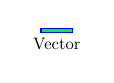
\begin{tikzpicture}[scale=0.1, every node/.style={transform shape}]
			\pgfmathsetmacro{\rectx}{4}
			\pgfmathsetmacro{\recty}{0.5}
			\draw[blue,fill=pastelgreen] (0,0) -- node [below, scale=6, black] {Vector}++(-\rectx,0) -- ++(0,\recty) -- ++(\rectx, 0) -- cycle;
			\end{tikzpicture}$\;$
			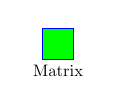
\begin{tikzpicture}[scale=0.1, every node/.style={transform shape}]
			\pgfmathsetmacro{\rectx}{4}
			\pgfmathsetmacro{\recty}{4}
			\draw[blue,fill=pastelgreen] (0,0) -- node [below, scale=6, black] {Matrix}++(-\rectx,0) -- ++(0,\recty) -- ++(\rectx, 0) -- cycle;
			%%\addvmargin{4};
			\end{tikzpicture}$\;$
			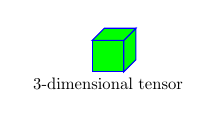
\begin{tikzpicture}[scale=0.1, every node/.style={transform shape}]
			\pgfmathsetmacro{\cubex}{4}
			\pgfmathsetmacro{\cubey}{4}
			\pgfmathsetmacro{\cubez}{4}
			\draw[blue,fill=pastelgreen] (0,0,0) -- ++(-\cubex,0,0) -- ++(0,-\cubey,0) --node [below, scale=6, black] {3-dimensional tensor} ++(\cubex,0,0) -- cycle;
			\draw[blue,fill=pastelgreen] (0,0,0) -- ++(0,0,-\cubez) -- ++(0,-\cubey,0) -- ++(0,0,\cubez) -- cycle;
			\draw[blue,fill=pastelgreen] (0,0,0) -- ++(-\cubex,0,0) -- ++(0,0,-\cubez) -- ++(\cubex,0,0) -- cycle;
			\end{tikzpicture}$\;$
			%%	\end{center}
			%%	\begin{center}	
			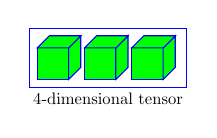
\begin{tikzpicture}[scale=0.1, every node/.style={transform shape}]
			\pgfmathsetmacro{\cubex}{4}
			\pgfmathsetmacro{\cubey}{4}
			\pgfmathsetmacro{\cubez}{4}
			\draw[blue,fill=pastelgreen] (0,0,0) -- ++(-\cubex,0,0) -- ++(0,-\cubey,0) -- ++(\cubex,0,0) -- cycle;
			\draw[blue,fill=pastelgreen] (0,0,0) -- ++(0,0,-\cubez) -- ++(0,-\cubey,0) -- ++(0,0,\cubez) -- cycle;
			\draw[blue,fill=pastelgreen] (0,0,0) -- ++(-\cubex,0,0) -- ++(0,0,-\cubez) -- ++(\cubex,0,0) -- cycle;
			
			\draw[blue,fill=pastelgreen] (\cubex +2,0,0) -- ++(-\cubex,0,0) -- ++(0,-\cubey,0) -- ++(\cubex,0,0) -- cycle;
			\draw[blue,fill=pastelgreen] (\cubex +2,0,0) -- ++(0,0,-\cubez) -- ++(0,-\cubey,0) -- ++(0,0,\cubez) -- cycle;
			\draw[blue,fill=pastelgreen] (\cubex +2,0,0) -- ++(-\cubex,0,0) -- ++(0,0,-\cubez) -- ++(\cubex,0,0) -- cycle;
			
			\draw[blue,fill=pastelgreen] (\cubex +2 + \cubex +2,0,0) -- ++(-\cubex,0,0) -- ++(0,-\cubey,0) -- ++(\cubex,0,0) -- cycle;
			\draw[blue,fill=pastelgreen] (\cubex +2 + \cubex +2,0,0) -- ++(0,0,-\cubez) -- ++(0,-\cubey,0) -- ++(0,0,\cubez) -- cycle;
			\draw[blue,fill=pastelgreen] (\cubex +2 + \cubex +2,0,0) -- ++(-\cubex,0,0) -- ++(0,0,-\cubez) -- ++(\cubex,0,0) -- cycle;
			
			\draw[blue, fill=none] (-\cubex -1, 2.5, 0) -- ++(0, -\cubey -3.5, 0) --node [below, scale=6, black] {4-dimensional tensor} ++(\cubex +2 + \cubex +2 + \cubex + \cubex,0,0) -- ++(0, \cubey +3.5, 0) -- cycle; 
			
			%%\node [scale=2] at (0, -8) {$hello$};
			\end{tikzpicture}
		\end{center}
	\end{minipage}
	%%\vspace*{-0.2cm}
	\vspace*{0.2cm}
	\begin{itemize}
		%%%%	\item \textbf{Cyber-Traffic}: IP x IP x Port x Time
		%%	\item[$\textcolor{blue}{\bullet}$] \textbf{Social-Network}: Person x Person x Time x Interaction-Type
		\item[$\textcolor{blue}{\bullet}$] \textbf{Social-Network}: Person x Person x Time x Type
	\end{itemize}
	
	\begin{itemize}
		\vfill
		\item High dimensional tensors: Neural network, Molecular simulation, Quantum computing
		\vfill
		\item People work with low dimensional structure (decomposition) of tensors
		\begin{center}
			\begin{columns}
				\hfill\begin{column}{0.34\linewidth}
					\begin{block}{\footnotesize Canonical decomposition}
						\begin{center}
							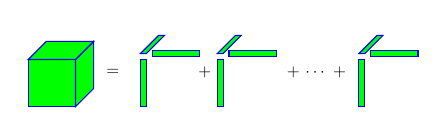
\begin{tikzpicture}[scale=0.15, every node/.style={transform shape}]
							%%						\pgfmathsetmacro{\cubex}{2}
							%%						\pgfmathsetmacro{\cubey}{2}
							%%						\pgfmathsetmacro{\cubez}{2}
							%%						\path (0,0,-\cubez-1) -- ++(-\cubex,0,0) -- ++(0,0,-\cubez-2) -- ++(\cubex,0,0) -- cycle;
							
							\path (-2,0,-7) -- (2,0,7);
							
							\pgfmathsetmacro{\cubex}{4}
							\pgfmathsetmacro{\cubey}{4}
							\pgfmathsetmacro{\cubez}{4}
							\draw[blue,fill=pastelgreen] (0,0,0) -- ++(-\cubex,0,0) -- ++(0,-\cubey,0) -- ++(\cubex,0,0) -- cycle;
							\draw[blue,fill=pastelgreen] (0,0,0) -- ++(0,0,-\cubez) -- ++(0,-\cubey,0) -- ++(0,0,\cubez) -- cycle;
							\draw[blue,fill=pastelgreen] (0,0,0) -- ++(-\cubex,0,0) -- ++(0,0,-\cubez) -- ++(\cubex,0,0) -- cycle;
							
							\node[draw=none, text=black, scale=4] at (2,-2.25,-3) {$=$};
							\pgfmathsetmacro{\smallwidth}{0.5}
							\draw[blue,fill=pastelgreen] (\cubex+2,0,0) -- ++(-\smallwidth,0,0) -- ++(0,-\cubey,0) -- ++(\smallwidth,0,0) -- cycle;
							\draw[blue,fill=pastelgreen] (\cubex+2 +\cubex + 0.5,0.75,0) -- ++(-\cubex,0,0) -- ++(0,-\smallwidth,0) -- ++(\cubex,0,0) -- cycle;
							\draw[blue,fill=pastelgreen] (\cubex+2,0.5,0) -- ++(-\smallwidth,0,0) -- ++(0,0,-\cubez) -- ++(\smallwidth,0,0) -- cycle;
							
							\node[draw=none, text=black, scale=4] at (2+\cubex+3.8,-2.25,-3) {$+$};
							
							\draw[blue,fill=pastelgreen] (\cubex+2.5 + \cubex+2,0,0) -- ++(-\smallwidth,0,0) -- ++(0,-\cubey,0) -- ++(\smallwidth,0,0) -- cycle;
							\draw[blue,fill=pastelgreen] (\cubex+2.5+\cubex+2 +\cubex + 0.5,0.75,0) -- ++(-\cubex,0,0) -- ++(0,-\smallwidth,0) -- ++(\cubex,0,0) -- cycle;
							\draw[blue,fill=pastelgreen] (\cubex+2.5+\cubex+2,0.5,0) -- ++(-\smallwidth,0,0) -- ++(0,0,-\cubez) -- ++(\smallwidth,0,0) -- cycle;
							
							\node[draw=none, text=black, scale=4] at (2+\cubex+5 + \cubex+ 4.25, -2.25,-3) {$+$ $\cdots$ $+$};
							
							\draw[blue,fill=pastelgreen] (12 + \cubex+2.5 + \cubex+2,0,0) -- ++(-\smallwidth,0,0) -- ++(0,-\cubey,0) -- ++(\smallwidth,0,0) -- cycle;
							\draw[blue,fill=pastelgreen] (12+\cubex+2.5+\cubex+2 +\cubex + 0.5,0.75,0) -- ++(-\cubex,0,0) -- ++(0,-\smallwidth,0) -- ++(\cubex,0,0) -- cycle;
							\draw[blue,fill=pastelgreen] (12 + \cubex+2.5+\cubex+2,0.5,0) -- ++(-\smallwidth,0,0) -- ++(0,0,-\cubez) -- ++(\smallwidth,0,0) -- cycle;
							\end{tikzpicture}
						\end{center}
					\end{block}
				\end{column}
				\begin{column}{0.265\linewidth}
					\begin{block}{\footnotesize Tucker decomposition}
						\begin{center}
							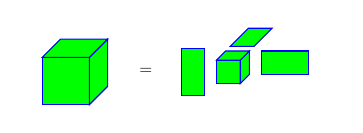
\begin{tikzpicture}[scale=0.15, every node/.style={transform shape}]
							\pgfmathsetmacro{\cubex}{4}
							\pgfmathsetmacro{\cubey}{4}
							\pgfmathsetmacro{\cubez}{4}
							\draw[blue,fill=pastelgreen] (-12,1,\cubez-2) -- ++(-\cubex,0,0) -- ++(0,-\cubey,0) -- ++(\cubex,0,0) -- cycle;
							\draw[blue,fill=pastelgreen] (-12,1,\cubez-2) -- ++(0,0,-\cubez) -- ++(0,-\cubey,0) -- ++(0,0,\cubez) -- cycle;
							\draw[blue,fill=pastelgreen] (-12,1,\cubez-2) -- ++(-\cubex,0,0) -- ++(0,0,-\cubez) -- ++(\cubex,0,0) -- cycle;
							\node[draw=none, text=black, scale=4] at (-8,-1,0) {$=$};
							
							\pgfmathsetmacro{\cubex}{2}
							\pgfmathsetmacro{\cubey}{2}
							\pgfmathsetmacro{\cubez}{2}
							\draw[blue,fill=pastelgreen] (0,0,0) -- ++(-\cubex,0,0) -- ++(0,-\cubey,0) -- ++(\cubex,0,0) -- cycle;
							\draw[blue,fill=pastelgreen] (0,0,0) -- ++(0,0,-\cubez) -- ++(0,-\cubey,0) -- ++(0,0,\cubez) -- cycle;
							\draw[blue,fill=pastelgreen] (0,0,0) -- ++(-\cubex,0,0) -- ++(0,0,-\cubez) -- ++(\cubex,0,0) -- cycle;
							
							\draw[blue,fill=pastelgreen] (-\cubex-1,1,0) -- ++(-\cubex,0,0) -- ++(0,-\cubey-2,0) -- ++(\cubex,0,0) -- cycle;
							\draw[blue,fill=pastelgreen] (\cubex+2+1,0,-\cubey) -- ++(-\cubex-2,0,0) -- ++(0,-\cubey,0) -- ++(\cubex+2,0,0) -- cycle;
							
							\draw[blue,fill=pastelgreen] (0,0,-\cubez-1) -- ++(-\cubex,0,0) -- ++(0,0,-\cubez-2) -- ++(\cubex,0,0) -- cycle;
							
							\path (-18,0) -- (8,0);
							\end{tikzpicture}
						\end{center}
					\end{block}
				\end{column}
				\begin{column}{0.265\linewidth}
					\begin{block}{\footnotesize Tensor-train decomposition}
						\begin{center}
							\begin{tikzpicture}[scale=0.15, every node/.style={transform shape}]
							
							\node (t0) at (0,-2.75) [scale=6] {$\tensor{X}$};
							\node [scale=4]at (2.5, -2.75) {$=$};
							\path (5,-6) -- (0,0);
							\end{tikzpicture}\hspace*{-0.15cm}
							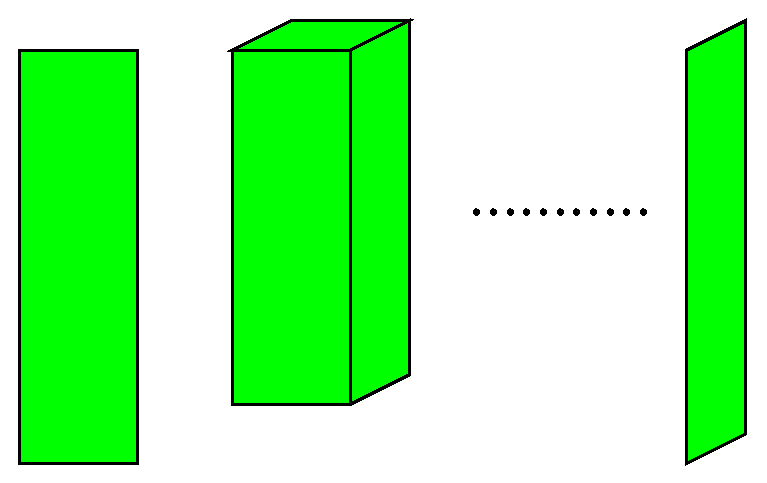
\includegraphics[scale=0.13]{./ttentry-simple.eps}
						\end{center}
						
					\end{block}
				\end{column}
			\end{columns}
		\end{center}
		
	\end{itemize}
	
\end{frame}

\begin{frame}{Importance of communication in high performance computing}
	\begin{minipage}{0.7\linewidth}
		\begin{itemize}	
			\item Gaps between computation and communication costs growing exponentially 
			%%	\item Gaps between computation and communication growing exponentially on a parallel computer
			%%{\footnotesize\begin{center}
			%%		\begin{tabular}{|c|c|c|c|}
			%%			\hline
			%%			& time-per-operation & Network-bandwidth & Network-latency\\ \hline
			%%			Annual improvements & 59 \% & 26 \% & 15 \%\\ \hline
			%%			%%		\multicolumn{2}{|c|}{Annual improvements}\\ \hline
			%%			%%		time-per-operation & 59\%\\ \hline
			%%			%%		Network-bandwidth & 26\%\\ \hline
			%%			%%		Network-latency & 15 \% \\ \hline
			%%		\end{tabular}$\qquad\qquad\qquad$
			%%\end{center}}
			{\footnotesize\begin{center}
					\begin{tabular}{|c|c|}
						\hline
						& Annual improvements\\ \hline
						Time-per-operation & 59 \%\\ \hline
						Network-bandwidth & 26 \%\\ \hline
						Network-latency & 15 \%\\ \hline
					\end{tabular}$\qquad\qquad\qquad$
			\end{center}}
			{$\ $\tiny Source: Getting up to speed: The future of supercomputing (observed from 2004)}
		\end{itemize}
	\end{minipage}
	\begin{minipage}{0.2\linewidth}
		\begin{center}
			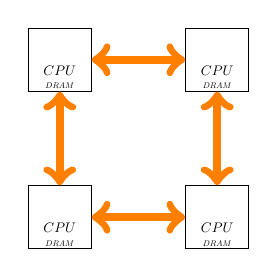
\begin{tikzpicture}[scale=0.5, every node/.style={transform shape}]
			%%\tikzstyle{taskmemory}=[draw=black, minimum height=18mm, minimum width=18mm, fill=blue!40, text=black]
			\tikzstyle{taskcompute}=[draw=black, minimum height=16mm, minimum width=16mm, fill=none, text=black, below]
			
			\node (t0) at (0,0) [taskcompute] {}; 
			\node (t1) at (4,0) [taskcompute] {};
			\node (t2) at (4,4) [taskcompute] {};
			\node (t3) at (0,4) [taskcompute] {};
			
			\draw [<->, line width=3, orange] (t0) -- (t1);
			\draw [<->, line width=3, orange] (t1) -- (t2);
			\draw [<->, line width=3, orange] (t2) -- (t3);
			\draw [<->, line width=3, orange] (t3) -- (t0);
			
			%%\draw [<->, line width=3, orange] (t0) -- (t2);
			%%\draw [<->, line width=3, orange] (t1) -- (t3);
			
			\node (td0)  at (t0.south) [above, scale=0.6] {$DRAM$};
			\node (td1) [above, scale=0.6] at (t1.south) {$DRAM$};
			\node (td2) [above, scale=0.6] at (t2.south) {$DRAM$};
			\node (td3) [above, scale=0.6] at (t3.south) {$DRAM$};
			
			\node [above] at (td0.north) {$CPU$};
			\node [above] at (td1.north) {$CPU$};
			\node [above] at (td2.north) {$CPU$};
			\node [above] at (td3.north) {$CPU$};
			\end{tikzpicture}
		\end{center}
	\end{minipage}
	\vfill
	\begin{block}{}
		\begin{itemize}
			\item \textbf{Goal}: Scalable and communication optimal tools for tensor computations
		\end{itemize}
	\end{block}
	
\end{frame}





\author[Suraj {\sc Kumar}]{\small Hussam {\sc Al Daas}\inst{1}, Grey {\sc Ballard}\inst{2}, Laura {\sc Grigori}\inst{3}, \underline{Suraj {\sc Kumar}}\inst{4}, Kathryn {\sc Rouse}\inst{5}, and  Mathieu {\sc Vérité}\inst{3}}

%%\underline{Suraj {\sc Kumar}}\inst{1}, Lionel {\sc Eyraud-Dubois}\inst{2}, and\\ Sriram {\sc Krishnamoorthy}\inst{1}}
\institute[ROMA team]{\inst{1} Rutherford Appleton Laboratory, UK \and %
	\inst{2} Wake Forest University, USA \and
	\inst{3} EPFL, Switzerland \and
	\inst{4} Inria and ENS Lyon, France \and
	\inst{5} Inmar Intelligence, USA}
\date[Jan 17, 2025]{Project committee meeting (Jan 17, 2025)} % Date, can be changed to a custom date
%\date{Jan 17, 2025} % Date, can be changed to a custom date


\begin{frame}
	\titlepage % Print the title page as the first slide
\end{frame}



%\begin{frame}{Completed (or Ongoing) research projects}
%	Communication optimal algorithms for 
%	\begin{itemize}
%		\vfill
%		\item[$\star$] \textcolor<2>{orange}{parallel Multiple Tensor-Times-Matrix (Multi-TTM) computation},
%		\vfill
%		\item[$\star$] symmetric matrix computations: SYRK ($C=AA^T$), SYR2K ($C=AB^T + BA^T$), and SYMM ($D=CB$ where $C$ is a symmetric matrix),
%		\vfill
%		\item parallel tensor-train decomposition, and
%		\vfill
%		\item[$\star$] \textcolor<2>{orange}{Nyström approximation with random matrices}.
%		\vfill
%		\vfill
%	\end{itemize}
%\vfill
%\scriptsize
%\only<1>{$\star$: with H.{\sc Al Daas} (Rutherford Appleton Laboratory, UK), G. {\sc Ballard} (Wake Forest University, USA), L. {\sc Grigori} (EPFL, Switzerland), K. {\sc Rouse} (Inmar Intelligence, USA), and M. {\sc Verite} (EPFL, Switzerland)}
%
%\end{frame}
	\section{Parallel Multiple Tensor-Times-Matrix (Multi-TTM) computation}
\begin{frame}{Outline}
		\tableofcontents[hideallsubsections]
		\vfill
		\vfill
		Our approach:
		\begin{itemize}
			\item Obtain communication lower bounds for each computation
			\item Design algorithms based on the communication lower bounds
		\end{itemize}
\end{frame}


\begin{frame}{Higher-order SVD (HOSVD) to compute Tucker decomposition}
		\begin{center}
		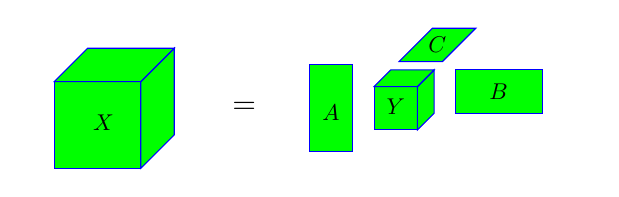
\begin{tikzpicture}[scale=0.275, every node/.style={transform shape}]
		\pgfmathsetmacro{\cubex}{4}
		\pgfmathsetmacro{\cubey}{4}
		\pgfmathsetmacro{\cubez}{4}
		\draw[blue,fill=pastelgreen] (-12,1,\cubez-2) -- ++(-\cubex,0,0) -- ++(0,-\cubey,0) -- ++(\cubex,0,0) -- cycle;
		\draw[blue,fill=pastelgreen] (-12,1,\cubez-2) -- ++(0,0,-\cubez) -- ++(0,-\cubey,0) -- ++(0,0,\cubez) -- cycle;
		\draw[blue,fill=pastelgreen] (-12,1,\cubez-2) -- ++(-\cubex,0,0) -- ++(0,0,-\cubez) -- ++(\cubex,0,0) -- cycle;
		\node [scale=3] at (-14.5,-1.65, 0) {$\X$};
		\node[draw=none, text=black, scale=4] at (-8,-1,0) {$=$};
		
		\pgfmathsetmacro{\cubex}{2}
		\pgfmathsetmacro{\cubey}{2}
		\pgfmathsetmacro{\cubez}{2}
		\draw[blue,fill=pastelgreen] (0,0,0) -- ++(-\cubex,0,0) -- ++(0,-\cubey,0) -- ++(\cubex,0,0) -- cycle;
		\draw[blue,fill=pastelgreen] (0,0,0) -- ++(0,0,-\cubez) -- ++(0,-\cubey,0) -- ++(0,0,\cubez) -- cycle;
		\draw[blue,fill=pastelgreen] (0,0,0) -- ++(-\cubex,0,0) -- ++(0,0,-\cubez) -- ++(\cubex,0,0) -- cycle;
		
		\node [scale=3] at (-1, -0.95, 0) {$\Y$};
		
		\draw[blue,fill=pastelgreen] (-\cubex-1,1,0) -- ++(-\cubex,0,0) -- ++(0,-\cubey-2,0) -- ++(\cubex,0,0) -- cycle;
		\node [scale=3] at (-4, -1.2, 0) {$A$};
		\draw[blue,fill=pastelgreen] (\cubex+2+1,0,-\cubey) -- ++(-\cubex-2,0,0) -- ++(0,-\cubey,0) -- ++(\cubex+2,0,0) -- cycle;
		\node [scale=3] at (3.75, -0.25, 0) {$B$};
		
		\draw[blue,fill=pastelgreen] (0,0,-\cubez-1) -- ++(-\cubex,0,0) -- ++(0,0,-\cubez-2) -- ++(\cubex,0,0) -- cycle;
		\node [scale=3] at (-1, 0, -5) {$C$};
		
		
		\path (-18,0) -- (8,0);
		\end{tikzpicture}
		
		{\footnotesize
			\begin{algorithm}[H]{\footnotesize
					\caption{3-dimensional HOSVD Algorithm($\X$)}
					%%				\caption{HOSVD Algorithm($\X$, $R_1$, $R_2$, $R_3$)}
					\begin{algorithmic}[1]
						%%					\STATE $A \leftarrow$ $R_1$ left singular vectors of $\X_{(1)}$
						%%					\STATE $B \leftarrow$ $R_2$ left singular vectors of $\X_{(2)}$
						%%					\STATE $C \leftarrow$ $R_3$ left singular vectors of $\X_{(3)}$
						\STATE Obtain factor matrices $A, B$ and $C$ from the matrix representations of the input tensor $\X$
						%%					 based on required accuracy
						\STATE $\Y = \X \times_1 A^\Tra \times_2 B^\Tra \times_3 C^\Tra$
						\STATE Return $\Y$, $A$, $B$, $C$
					\end{algorithmic}
			}\end{algorithm}
			
			\vspace*{-0.15cm}
			\begin{itemize}
				\item $\X$, $\Y$: 3-dimensional input and output tensors (or arrays) \& $A$, $B$, $C$: matrices
				\vfill
				%%			\item $\X_{(i)}$: matricization of $\X$ ($i$th dimension represents rows and remaining dimensions represent columns)
				\item $\times_i$: tensor contraction along the $i$th dimension (similar to matrix multiplication)
				\vfill
				\item Multiple Tensor-Times-Matrix (Multi-TTM) computation: $\Y = \X \times_1 A^\Tra \times_2 B^\Tra \times_3 C^\Tra$
				\vfill
				\item When $A, B$ and $C$ are obtained using randomized approaches, Multi-TTM becomes the bottleneck
				%%			\begin{itemize}
				%%				\item To obtain full tensor, $\X = \Y \times_1 A \times_2 B \times_3 C$
				%%			\end{itemize}
			\end{itemize}
			\vfill
		}
	\end{center}
\end{frame}

\begin{frame}{Multi-TTM: $\Y = \X \times_1 A^\Tra \times_2 B^\Tra \times_3 C^\Tra$}
	\begin{center}
		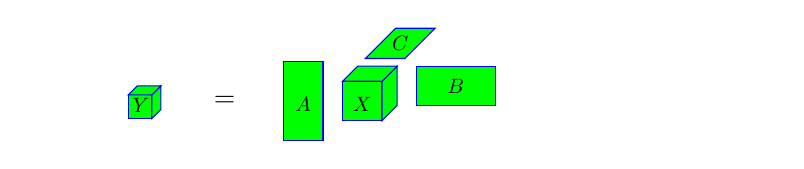
\begin{tikzpicture}[scale=0.25, every node/.style={transform shape}]
		\pgfmathsetmacro{\cubex}{1.2}
		\pgfmathsetmacro{\cubey}{1.2}
		\pgfmathsetmacro{\cubez}{1.2}
		\draw[blue,fill=pastelgreen] (-12,-1,\cubez-2) -- ++(-\cubex,0,0) -- ++(0,-\cubey,0) -- ++(\cubex,0,0) -- cycle;
		\node [scale=3] at (-12.25,-1.25, 0) {$\Y$};
		\draw[blue,fill=pastelgreen] (-12,-1,\cubez-2) -- ++(0,0,-\cubez) -- ++(0,-\cubey,0) -- ++(0,0,\cubez) -- cycle;
		\draw[blue,fill=pastelgreen] (-12,-1,\cubez-2) -- ++(-\cubex,0,0) -- ++(0,0,-\cubez) -- ++(\cubex,0,0) -- cycle;
		\node[draw=none, text=black, scale=4] at (-8,-1,0) {$=$};
		
		\pgfmathsetmacro{\cubex}{2}
		\pgfmathsetmacro{\cubey}{2}
		\pgfmathsetmacro{\cubez}{2}
		\draw[blue,fill=pastelgreen] (0,0,0) -- ++(-\cubex,0,0) -- ++(0,-\cubey,0) -- ++(\cubex,0,0) -- cycle;
		\draw[blue,fill=pastelgreen] (0,0,0) -- ++(0,0,-\cubez) -- ++(0,-\cubey,0) -- ++(0,0,\cubez) -- cycle;
		\draw[blue,fill=pastelgreen] (0,0,0) -- ++(-\cubex,0,0) -- ++(0,0,-\cubez) -- ++(\cubex,0,0) -- cycle;
		
		\node [scale=3] at (-1, -1.2, 0) {$\X$};
		\draw[blue,fill=pastelgreen] (-\cubex-1,1,0) -- ++(-\cubex,0,0) -- ++(0,-\cubey-2,0) -- ++(\cubex,0,0) -- cycle;
		
		\node [scale=3] at (-4, -1.2, 0) {$A$};
		
		\draw[blue,fill=pastelgreen] (\cubex+2+1,0,-\cubey) -- ++(-\cubex-2,0,0) -- ++(0,-\cubey,0) -- ++(\cubex+2,0,0) -- cycle;
		\node [scale=3] at (3.75, -0.25, 0) {$B$};
		
		\draw[blue,fill=pastelgreen] (0,0,-\cubez-1) -- ++(-\cubex,0,0) -- ++(0,0,-\cubez-2) -- ++(\cubex,0,0) -- cycle;
		\node [scale=3] at (-1, 0, -5) {$C$};
		
		\path (-18,0) -- (20,0);
		\end{tikzpicture}
	\end{center}
	\begin{itemize}
		\item Focus on communication cost of Multi-TTM on a parallel homogeneous machine
		\vfill
		\item Multi-TTM is also the bottleneck computation for Sequentially Truncated HOSVD
	\end{itemize}
	\begin{block}{Settings}
		\begin{itemize}
			\item $P$ number of processors
			\item Each processor performs (asymptotically) equal amount of operations
			%%		\item No redundant operations
			\item One copy of data is in the system
			\item Focus on bandwidth cost (volume of data transfers)
		\end{itemize}
	\end{block}
	
	\vfill
	{\footnotesize H. Al Daas, G. Ballard, L. Grigori, S. Kumar, and K. Rouse, \emph{Communication lower bounds and optimal algorithms
			for multiple tensor-times-matrix computation}, SIMAX, 2024.}
\end{frame}

\subsection{Our approach to compute communication lower bounds}
\subsubsection{For Traditional Matrix Matrix Multiplication}
\begin{frame}{Outline}
	%	\tableofcontents[hidesubsections] 
	\tableofcontents[currentsubsection]
\end{frame}

\begin{frame}{Approach to obtain communication lower bounds}
	
	{\small
		\begin{minipage}{0.7\linewidth}
			\begin{itemize}
				\item Loomis-Whitney inequalitiy: for $d-1$ dimensional projections
				\begin{itemize}
					\item For the $2$d object $A$, $\phi_x \phi_y \ge Area(A)$
					\item For the $3$d object $B$, $(\phi_{xy}\phi_{yz}\phi_{xz})^\frac{1}{2} \ge Volume(B)$
					%%		\item $2$-dimensional object $A$ and its $1$-dimensional projections are $\phi_x$ and $\phi_y$, then $\phi_x \phi_y \ge Area(A)$
					%%		\item $3$-dimensional object $B$ and its $2$-dimensional projections are $\phi_{xy}$, $\phi_{yz}$ and $\phi_{xz}$, then $(\phi_{xy}\phi_{yz}\phi_{xz})^\frac{1}{2} \ge Volume(B)$
				\end{itemize}
			\end{itemize}
		\end{minipage}$\quad$
		\begin{minipage}{0.25\linewidth}
			\begin{center}
				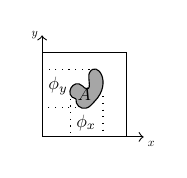
\begin{tikzpicture}[scale=0.215, every node/.style={transform shape}]
				\draw (0,0) -- ++(5,0) -- ++(0, 5) -- ++(-5,0) -- cycle;
				\draw [<->] (0,6) -- (0,0) -- (6,0);
				\node [below right, scale=2] at (6,0) {$x$};
				\node [left, scale=2] at (0,6) {$y$};
				
				\draw [fill=gray!70] (2,2.25) to [curve through={(2.4,3) .. (2.5,2.9) .. (2.8,3.8) .. (3.1,2.1) .. (2.6,1.7)}] (2,2.25);
				
				\node [scale=3] at (2.5,2.5) {$A$};
				\draw [dotted] (1.7,2.25) -- (1.7,0);
				\draw [dotted] (3.6,2.4) -- (3.6,0);
				
				\node[above, scale=3] at (2.6,0) {$\phi_x$};
				
				\draw [dotted] (2,1.75) -- (0,1.75);
				\draw [dotted] (2.8,4) -- (0,4);
				
				\node[right, scale=3] at (0,3) {$\phi_y$};
				\end{tikzpicture}
				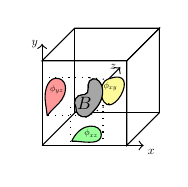
\begin{tikzpicture}[scale=0.215, every node/.style={transform shape}]
				\draw (0,0) -- ++(5,0) -- ++(0, 5) -- ++(-5,0) -- cycle;
				\draw (0,5,0) -- ++(0,0, -5) -- ++(5,0,0) -- ++(0,0,5) -- cycle;
				\draw (5,0,0) -- ++(0,0,-5) -- ++(0,5,0) -- ++(0,0,5) -- cycle;
				\draw (0,0,-5) -- ++(5,0,0) -- ++(0,5,0) -- ++(-5,0,0) -- cycle;
				\draw [<->] (0,6) -- (0,0) -- (6,0);
				\draw [->] (0,0,0) -- (0,0,-12);
				\node [left, scale=2, rotate=0] at (0,0,-12) {$z$};
				\node [below right, scale=2] at (6,0) {$x$};
				\node [left, scale=2] at (0,6) {$y$};
				
				\draw [fill=gray!70] (2,2.25) to [curve through={(2.4,3) .. (2.5,3) .. (2.8,3.8) .. (3.1,2.1) .. (2.6,1.7)}] (2,2.25);
				
				\node [scale=2] at (2.5,2.5) {$A$};
				\draw [dotted] (1.7,2.25) -- (1.7,0.2);
				\draw [dotted] (3.6,2.4) -- (3.6,0.3);
				
				\draw [fill=green!40] (1.75,0.25) to [curve through={(1.8, 0.35) .. (3.5, 0.65) .. (2,0.25)}] (1.75,0.25);
				\node[above, scale=1.5] at (2.6,0,-0.75) {$\phi_{xz}$};
				
				\draw [dotted] (2,1.75) -- (0.3,1.75);
				\draw [dotted] (2.8,4) -- (0.385,4);
				
				\draw [fill=red!40] (0.3, 1.75) to [curve through={(0.5,2) .. (1, 2.5) .. (1,3.95) .. (0.2, 2.5)}] (0.3,1.75);
				\node[right, scale=1.5] at (0,3, -0.75) {$\phi_{yz}$};
				
				\draw [fill=yellow!40] (3.85,3.9) to [curve through={(3.7,3.8) .. (3.5,3.4) .. (3.45,3.2)}] (3.85, 3.9);
				\node [scale=1.5] at (3.65,3.1,-1) {$\phi_{xy}$};
				\draw [dotted] (2.8,4) -- (3.8,3.9);
				\draw [dotted] (2.56,1.65) -- (4,2.5);
				
				\draw [fill=gray!70] (2,2.25) to [curve through={(2.4,3) .. (2.5,3) .. (2.8,3.8) .. (3.1,2.1) .. (2.6,1.7)}] (2,2.25);
				
				\node [scale=3] at (2.5,2.5) {$B$};
				\end{tikzpicture}
			\end{center}
		\end{minipage}
		\begin{itemize}
			\item H\"{o}lder-Brascamp-Lieb (HBL) inequality -- generalization for arbitrary dimensional projections
			\begin{itemize}
				\item Provide exponent for each projection
				%%		\item Work with $\M{\Delta}$ matrix that depends on the array accesses
				%%		\item $\V{1}$ is vector of all ones and $\M{\Delta}$ depends on the array accesses in the computation
				%%		\item $\V{x}$ and projections provide relation with the amount of computations 
			\end{itemize}
		\end{itemize}
		\vspace*{-0.15cm}
		\begin{block}{\small Constraints for parallel load balanced matrix matrix multiplication}
			\begin{itemize}
				\item $C=AB$ with $A \in \mathbb{R}^{n_1\times n_2}, B \in \mathbb{R}^{n_2\times n_3}$, and $C \in \mathbb{R}^{n_1\times n_3}$
			\end{itemize}
			\vspace*{-0.45cm}\begin{align*}
			&\text{for $i = 1{:}n_1$, for $k = 1{:}n_2$, for $j = 1{:}n_3$}\\
			&\quad \quad C[i][j] += A[i][k]*B[k][j]
			\end{align*}
			%%\begin{columns}
			%%	\begin{column}{0.35\linewidth}{\small
			%%			\vspace*{-0.425cm}\begin{center}
			%%				$\M{\Delta} = \begin{blockarray}{cccc}
			%%				& A & B & C  \\
			%%				\begin{block}{c(ccc)}
			%%				i & 1 & 0 & 1\\
			%%				j & 0 & 1 & 1\\
			%%				k & 1 & 1 & 0\\
			%%				\end{block}
			%%				\end{blockarray}$
			%%			\end{center}
			%%	}\end{column}
			%%	\begin{column}{0.6\linewidth}
			%%		\vspace*{-0.35cm}\begin{align*}
			%%		&\text{for $i = 1{:}n_1$, for $k = 1{:}n_2$, for $j = 1{:}n_3$}\\
			%%		&\quad \quad C[i][j] += A[i][k]*B[k][j]
			%%		\end{align*}
			%%	\end{column}
			%%\end{columns}
			%%\vspace*{-0.2cm}
			\begin{itemize}[leftmargin=5.5mm]
				%%	\item For tight bounds, find vector $\V{x}$ such that $\M{\Delta}.\V{x} = \V{1}$
				%%	\item $\phi_A, \phi_B, \phi_C$: projections of computations on arrays $A$, $B$, $C$ and $\V{x}=\begin{bmatrix} \frac{1}{2} & \frac{1}{2} & \frac{1}{2} \end{bmatrix}^\Tra$
				\item $\phi_A, \phi_B, \phi_C$: projections of computations on arrays $A$, $B$, $C$
				\item From Loomis-Whitney/HBL inequality: $\phi_A^{\frac{1}{2}} \phi_B^{\frac{1}{2}} \phi_C^{\frac{1}{2}} \ge \text{number of multiplications per processor}=\frac{n_1n_2n_3}{P}$
				\item Extra constraints: $\frac{n_1n_2}{P} \le \phi_A \le n_1n_2$, $\frac{n_2n_3}{P} \le \phi_B \le n_2n_3$, $\frac{n_1n_3}{P} \le \phi_C \le n_1n_3$
			\end{itemize}
		\end{block}
	}
\end{frame}



\begin{frame}{Optimization problem and communication lower bounds}
	
	{\footnotesize 
		%%		\begin{itemize}
		%%			\item $\phi_A,  \phi_B, \phi_C$ indicate the amount of array accesses
		%%		\end{itemize}
		\begin{center}
			\vspace*{-0.375cm}\begin{align*}
			Minimize &\ \phi_A + \phi_B + \phi_C \  \text{ s.t.}\\
			\phi_A^\frac{1}{2} \phi_B^\frac{1}{2}  \phi_C^\frac{1}{2} & \ge \frac{n_1n_2n_3}{P}\\
			\frac{n_1n_2}{P} \le &\phi_A \le n_1n_2\\
			\frac{n_2n_3}{P} \le &\phi_B \le n_2n_3\\
			\frac{n_1n_3}{P} \le &\phi_C \le n_1n_3
			\end{align*}
		\end{center}
		
		%%\vfill
		\vspace*{-0.15cm}
		\begin{block}{\footnotesize Amount of array accesses = $\phi_A + \phi_B + \phi_C$}
			%%	\begin{block}{}
			%%$\bullet$ Estimate the solution based on Lagrange multipliers\\
			%%$\bullet$ Prove optimality using all Karush–Kuhn–Tucker (KKT) conditions are satisfied
			$\bullet$ Estimate the solution and prove optimality by showing Karush--Kuhn--Tucker (KKT) conditions are satisfied\\
			$\bullet$ For $n_1\le n_2\le n_3$,
			%%$\bullet$ Prove optimality using all Karush–Kuhn–Tucker (KKT) conditions are satisfied
			\vspace*{-0.1cm}\begin{center}
				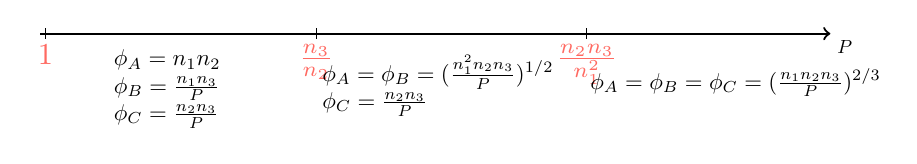
\begin{tikzpicture}[scale=0.6875, every node/.style={transform shape}]
				%%\draw (-2,0) -- node[below] {a} ++(2,0) -- node[above] {b} ++(2,0);
				%%\draw (-0.1,0) -- ++(5,0) -- ++(5,0);
				\draw [->, thick] (-0.1,0) -- (14.5,0) node [below right] {$P$};
				\draw (0, 0.1) -- node [below, pastelred, scale=1.6]{$1$}(0,-0.1);
				\draw (5, 0.1) -- node [below, pastelred, scale=1.6]{$\frac{n_3}{n_2}$}(5,-0.1);
				\draw (10, 0.1) -- node [below, pastelred, scale=1.6] {$\frac{n_2n_3}{n_1^2}$}(10,-0.1);
				
				\node[align=left,below,scale=1.2] at (2.25, -0.15) {$\phi_A = n_1n_2$\\ $\phi_B=\frac{n_1n_3}{P}$\\ $\phi_C = \frac{n_2n_3}{P}$};
				\node[align=left,below,scale=1.2] at (7.25, -0.25) {$\phi_A =\phi_B= (\frac{n_1^2n_2n_3}{P})^{1/2}$\\ $\phi_C = \frac{n_2n_3}{P}$};
				\node[align=center,below,scale=1.2] at (12.75, -0.5) {$\phi_A = \phi_B = \phi_C = (\frac{n_1n_2n_3}{P})^{2/3}$};	
				\end{tikzpicture}
			\end{center}\vspace*{-0.25cm}
			$\bullet$ Communication lower bound = $\phi_A + \phi_B + \phi_C - \text{data owned by the processor} = \phi_A + \phi_B + \phi_C - \frac{n_1n_2+n_2n_3+n_1n_3}{P}$
		\end{block}	
	}
\end{frame}




\subsubsection{For Multi-TTM Computation}
\begin{frame}{Outline}
	\tableofcontents[currentsubsection]
\end{frame}

\begin{frame}{3-dimensional Multi-TTM computation}
	
	\begin{columns}
		\begin{column}{0.435\linewidth}
			\begin{center}
				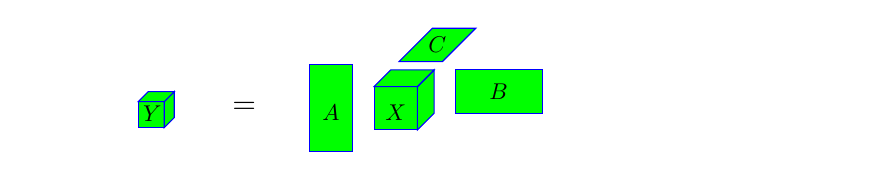
\begin{tikzpicture}[scale=0.275, every node/.style={transform shape}]
				\pgfmathsetmacro{\cubex}{1.2}
				\pgfmathsetmacro{\cubey}{1.2}
				\pgfmathsetmacro{\cubez}{1.2}
				\draw[blue,fill=pastelgreen] (-12,-1,\cubez-2) -- ++(-\cubex,0,0) -- ++(0,-\cubey,0) -- ++(\cubex,0,0) -- cycle;
				\node [scale=3] at (-12.25,-1.25, 0) {$\Y$};
				\draw[blue,fill=pastelgreen] (-12,-1,\cubez-2) -- ++(0,0,-\cubez) -- ++(0,-\cubey,0) -- ++(0,0,\cubez) -- cycle;
				\draw[blue,fill=pastelgreen] (-12,-1,\cubez-2) -- ++(-\cubex,0,0) -- ++(0,0,-\cubez) -- ++(\cubex,0,0) -- cycle;
				\node[draw=none, text=black, scale=4] at (-8,-1,0) {$=$};
				
				\pgfmathsetmacro{\cubex}{2}
				\pgfmathsetmacro{\cubey}{2}
				\pgfmathsetmacro{\cubez}{2}
				\draw[blue,fill=pastelgreen] (0,0,0) -- ++(-\cubex,0,0) -- ++(0,-\cubey,0) -- ++(\cubex,0,0) -- cycle;
				\draw[blue,fill=pastelgreen] (0,0,0) -- ++(0,0,-\cubez) -- ++(0,-\cubey,0) -- ++(0,0,\cubez) -- cycle;
				\draw[blue,fill=pastelgreen] (0,0,0) -- ++(-\cubex,0,0) -- ++(0,0,-\cubez) -- ++(\cubex,0,0) -- cycle;
				
				\node [scale=3] at (-1, -1.2, 0) {$\X$};
				\draw[blue,fill=pastelgreen] (-\cubex-1,1,0) -- ++(-\cubex,0,0) -- ++(0,-\cubey-2,0) -- ++(\cubex,0,0) -- cycle;
				
				\node [scale=3] at (-4, -1.2, 0) {$A$};
				
				\draw[blue,fill=pastelgreen] (\cubex+2+1,0,-\cubey) -- ++(-\cubex-2,0,0) -- ++(0,-\cubey,0) -- ++(\cubex+2,0,0) -- cycle;
				\node [scale=3] at (3.75, -0.25, 0) {$B$};
				
				\draw[blue,fill=pastelgreen] (0,0,-\cubez-1) -- ++(-\cubex,0,0) -- ++(0,0,-\cubez-2) -- ++(\cubex,0,0) -- cycle;
				\node [scale=3] at (-1, 0, -5) {$C$};
				
				\path (-18,0) -- (20,0);
				\end{tikzpicture}
			\end{center}
		\end{column}
		\begin{column}{0.56\linewidth}
			\begin{itemize} {\footnotesize
					%%				\item Used to compute Tucker decomposition 
					\item $\Y = \X \times_1 A^\Tra \times_2 B^\Tra \times_3 C^\Tra$
					\item $\X$, $\Y$: 3-dimensional input and output tensors
					\item $A, B, C$: matrices
					\item $\times_i$: analogous to matrix multiplication
					
					%%		\item $\times_i$: tensor contraction along the $i$th dimension (similar to matrix multiplication)
			}\end{itemize}
		\end{column}
	\end{columns}
	\vfill
	\begin{itemize}
		%%	\item 3-dimensional Multi-TTM ($\Y = \X \times_1 {\Mn{A}{1}}^\Tra \times_2 {B}^\Tra \times_3 {\Mn{A}{3}}^\Tra$)
		\item TTM-in-Sequence approach (used in TuckerMPI library):
		$\Y = \left(\left(\X \times_1 A^\Tra \right)\times_2 B^\Tra \right)\times_3 C^\Tra$
		\vfill
		\item Our All-at-Once definition with {\small$\X \in \mathbb{R}^{n_1\times n_2\times n_3}$, $\Y\in \mathbb{R}^{r_1 \times r_2 \times r_3}$, $A\in \mathbb{R}^{n_1\times r_1}$, $B\in \mathbb{R}^{n_2\times r_2}$, $C\in \mathbb{R}^{n_3\times r_3}$
			%%			\vspace*{-0.15cm}\begin{align*}
			%%			&\text{for $n_1^\prime = 1{:}n_1$, for $n_2^\prime = 1{:}n_2$, for $n_3^\prime = 1{:}n_3$}\\
			%%			&\quad \text{for $r_1^\prime = 1{:}r_1$, for $r_2^\prime = 1{:}r_2$, for $r_3^\prime = 1{:}r_3$}\\
			%%			&\quad \quad \Y(r_1^\prime,r_2^\prime,r_3^\prime) = \Y(r_1^\prime,r_2^\prime,r_3^\prime)\\
			%%			&\qquad\qquad\quad + \Big( \X(n_1^\prime,n_2^\prime,n_3^\prime) *  \Mn{A}{1}(n_{1}^\prime,r_1^\prime) * B(n_2^\prime,r_2^\prime) * \Mn{A}{3}(n_3^\prime,r_3^\prime)\Big)
			%%			\end{align*}\vspace*{-0.5cm}
			\begin{align*}
			&\text{for \{$n_1^\prime, n_2^\prime, n_3^\prime, r_1^\prime, r_2^\prime, r_3^\prime$\}} = 1{:}\text{\{$n_1,n_2,n_3,r_1,r_2,r_3$\}}\\
			&\quad  \Y(r_1^\prime,r_2^\prime,r_3^\prime) += \X(n_1^\prime,n_2^\prime,n_3^\prime) \cdot  A(n_{1}^\prime,r_1^\prime) \cdot B(n_2^\prime,r_2^\prime) \cdot C(n_3^\prime,r_3^\prime)
			\end{align*}\vspace*{-0.5cm}
		}
		%		\vfill
		%		\item Establish lower bounds on data transfers based on the geometry of computations
		%		\vfill
		%		\item Design a $6$-dimensional parallel algorithm
		%		\begin{itemize}
		%			\item Select right parameters based on lower bounds to achieve communication optimality
		%		\end{itemize}
		%		\vfill
	\end{itemize}
\end{frame}

\setcounter{algorithm}{0}
\begin{frame}{Solving optimization problems to compute lower bounds}
	\begin{itemize}
		\item Each processor performs $\frac{n_1r_1n_2r_2n_3r_3}{P}$ amount of $4-array$ operations
		\item After applying lower and upper bounds for each projection, we need to solve the following optimization problem
	\end{itemize}
	\vspace*{-0.35cm}{\small\begin{align*}
		Minimize \ \phi_{\X} + \phi_{\Y} +& \phi_1 + \phi_2 + \phi_3 \  \text{ s.t.}\\
		\phi_{\X}^{1-a}\phi_{\Y}^{1-a} \phi_1^a \phi_2^a \phi_3^a & \ge \frac{n_1r_1n_2r_2n_3r_3}{P}\\
		\frac{n_1n_2n_3}{P} \le & \phi_{\X} \le n_1n_2n_3\\
		\frac{r_1r_2r_3}{P} \le & \phi_{\Y} \le r_1r_2r_3\\
		\frac{n_1r_1}{P} \le &\phi_1 \le n_1r_1\\
		\frac{n_2r_2}{P} \le &\phi_2 \le n_2r_2\\
		\frac{n_3r_3}{P} \le &\phi_3 \le n_3r_3\\
		0 \le & a \le 1
		\end{align*}}
\end{frame}
\begin{frame}{Divide the problem into two parts}
	\vspace*{-0.25cm}
	\begin{minipage}{0.45\linewidth}
		\begin{block}{Matrix part}{\small
				\vspace*{-0.45cm}\begin{align*}
				Minimize \ & \phi_1 + \phi_2 + \phi_3 \  \text{ s.t.}\\
				\phi_1 \phi_2 \phi_3 & \ge \frac{n_1r_1n_2r_2n_3r_3}{P}\\
				\frac{n_1r_1}{P} \le &\phi_1 \le n_1r_1\\
				\frac{n_2r_2}{P} \le &\phi_2 \le n_2r_2\\
				\frac{n_3r_3}{P} \le &\phi_3 \le n_3r_3
				\end{align*}
		}\end{block}
	\end{minipage}$\quad$
	\begin{minipage}{0.45\linewidth}
		\begin{block}{Tensor part}{\small
				\begin{align*}
				Minimize \ & \phi_{\X} + \phi_{\Y}\  \text{ s.t.}\\
				\phi_{\X}\phi_{\Y} & \ge \frac{n_1r_1n_2r_2n_3r_3}{P}\\
				\frac{n_1n_2n_3}{P} \le & \phi_{\X} \le n_1n_2n_3\\
				\frac{r_1r_2r_3}{P} \le & \phi_{\Y} \le r_1r_2r_3
				\end{align*}
		}\end{block}
	\end{minipage}
	
	
\end{frame}
\begin{frame}{Amount of accesses and lower bounds}
	\begin{itemize}{\small
			\item We assume $n_1r_1\le n_2r_2\le n_3r_3$ and $r_1r_2r_3\le n_1n_2n_3$
			\item Estimate the solutions and prove optimality by showing  KKT conditions are satisfied
	}\end{itemize}
	\vspace*{-0.25cm}\begin{block}{Amount of accesses = $\phi_{\X} + \phi_{\Y} + \phi_1 + \phi_2 + \phi_3$}
		\begin{center}
			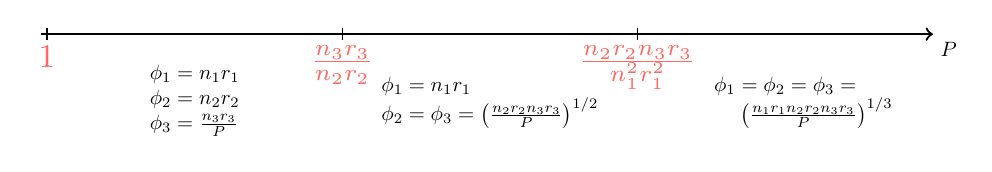
\begin{tikzpicture}[scale=0.75, every node/.style={transform shape}]
			%%\draw (-2,0) -- node[below] {a} ++(2,0) -- node[above] {b} ++(2,0);
			%%\draw (-0.1,0) -- ++(5,0) -- ++(5,0);
			\draw [->, thick] (-0.1,0) -- (15,0) node [below right] {$P$};
			\draw (0, 0.1) -- node [below, pastelred, scale=1.6]{$1$}(0,-0.1);
			\draw (5, 0.1) -- node [below, pastelred, scale=1.6]{$\frac{n_3r_3}{n_2r_2}$}(5,-0.1);
			\draw (10, 0.1) -- node [below, pastelred, scale=1.6] {$\frac{n_2r_2n_3r_3}{n_1^2r_1^2}$}(10,-0.1);
			
			\node[align=left,below] at (2.5, -0.4) {$\phi_1=n_1r_1$\\ $\phi_2=n_2r_2$\\ $\phi_3=\frac{n_3r_3}{P}$};
			\node[align=left,below] at (7.5, -0.6) {$\phi_1=n_1r_1$\\$\phi_2=\phi_3= \big(\frac{n_2r_2n_3r_3}{P}\big)^{1/2}$};
			\node[align=center,below] at (12.5, -0.6) {$\phi_1=\phi_2=\phi_3=$\\ $\qquad\quad \big(\frac{n_1r_1n_2r_2n_3r_3}{P}\big)^{1/3}$};	
			\end{tikzpicture}
		\end{center}
		
		\begin{center}
			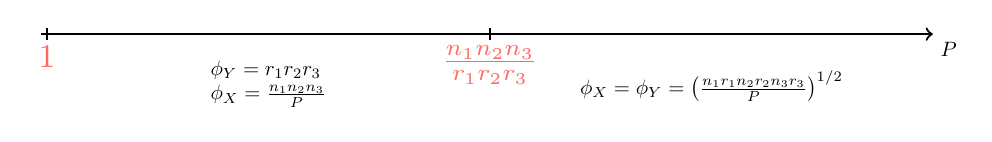
\begin{tikzpicture}[scale=0.75, every node/.style={transform shape}]
			\draw [->, thick] (-0.1,0) -- (15,0) node [below right] {$P$};
			\draw (0, 0.1) -- node [below, pastelred, scale=1.6]{$1$}(0,-0.1);
			\draw (7.5, 0.1) -- node [below, pastelred, scale=1.6]{$\frac{n_1n_2n_3}{r_1r_2r_3}$}(7.5,-0.1);
			
			\node[align=left,below] at (3.75, -0.325) {$\phi_{\Y}= r_1r_2r_3$\\ $\phi_{\X} = \frac{n_1n_2n_3}{P}$};
			\node[align=left,below] at (11.25, -0.5) {$\phi_{\X}=\phi_{\Y}= \big(\frac{n_1r_1n_2r_2n_3r_3}{P}\big)^{1/2}$};
			\end{tikzpicture}
		\end{center}
	\end{block}
	Communication lower bound = $\phi_{\X} + \phi_{\Y} + \phi_1 + \phi_2 + \phi_3 -\frac{n_1n_2n_3+r_1r_2r_3+n_1r_1+n_2r_2+n_3r_3}{P}$
\end{frame}

\subsection{Communication Optimal Algorithm and Simulated Experiments}
\begin{frame}{Outline}
	\tableofcontents[currentsubsection]
\end{frame}
\begin{frame}{Design of communication optimal algorithms}
	\begin{block}{\small Data Distribution ($P$ is organized into a $p_1 \times p_2 \times p_3\times q_1 \times q_2 \times q_3$ grid)}{\small
			%%		\begin{minipage}{0.75\linewidth}{\small	
			\begin{itemize}
				\item $p_1,p_2, p_3, q_1, q_2$, and $q_3$ evenly distribute $n_1, n_2, n_3, r_1, r_2$, and  $r_3$
				\item Each processor has $\frac{1}{P}$th amount of input and output variables
				\item Subtensor $\T{X}_{231} = \T{X}(\frac{n_1}{p_1}+1:2\frac{n_1}{p_1}, 2\frac{n_2}{p_2}+1:3\frac{n_2}{p_2}, 1:\frac{n_3}{p_3})$ is distributed evenly among processors $(2,3,1,*,*,*)$ 
				\item Submatrix $B_{31} = B(2\frac{n_2}{p_2}+1:3\frac{n_2}{p_2}, 1:\frac{r_2}{q_2})$ is distributed evenly among processors $(*,3,*,*,1,*)$
			\end{itemize}
			%%		}\end{minipage}
			\begin{center}
				\vspace*{-0.25cm}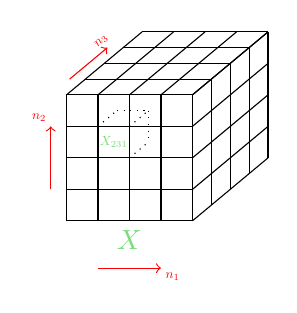
\begin{tikzpicture}[scale=0.4, every node/.style={transform shape}]
				\def\xref{0.6}
				\def\yref{0.5}
				
				\foreach \y in {0, 1, 2, 3, 4}
				\draw (-2, \y) -- (2, \y);
				
				\foreach \x in {-2, -1, 0, 1, 2}
				\draw (\x, 0) -- (\x, 4);
				
				\foreach \y in {0, 1, 2, 3, 4}
				\draw (2, \y)--(2+4*\xref, 4*\yref+\y);
				
				
				\foreach \y in {0, 1, 2, 3, 4}
				\draw (2+\y * \xref, \y * \yref) -- (2+\y * \xref, 4+\y * \yref);
				
				\foreach \x in {-2, -1, 0, 1, 2}
				\draw (\x, 4) -- (\x + 4*\xref, 4+4*\yref);
				
				\foreach \y in {0, 1, 2, 3, 4}
				\draw (-2+\y * \xref, 4+\y * \yref) -- (2+\y * \xref, 4+\y * \yref);
				
				\node [below, pastelgreen1, scale=2.5] at (0,0) {$\T{X}$};
				
				\draw [dotted] (-1, 3) -- (-1+\xref,3+\yref);
				\draw [dotted] (0, 3) -- (0+\xref,3+\yref);
				\draw [dotted] (0, 2) -- (0+\xref,2+\yref);
				\draw [dotted] (-1+\xref,3+\yref) -- (0+\xref,3+\yref);
				\draw [dotted] (0+\xref,3+\yref) -- (0+\xref,2+\yref);
				
				\node [pastelgreen1, scale=1.2] at (-0.5,2.5) {$\T{X}_{231}$};
				
				\draw [->, red] (-1,-1.5) -- (1,-1.5) node [below right, scale=1.2] {$n_1$};
				\draw [->, red] (-2.5,1) -- (-2.5,3) node [ above left, scale=1.2] {$n_2$};
				\draw [->, red] (-2.5+\xref, 4+\yref) -- (-2.5 + 3*\xref, 4+3*\yref) node [above,rotate=45, scale=1.2] {$n_3$};
				\end{tikzpicture}$\qquad$
				\vspace*{-0.25cm}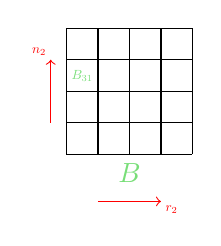
\begin{tikzpicture}[scale=0.4, every node/.style={transform shape}]
				\def\xref{0.6}
				\def\yref{0.5}
				
				\foreach \y in {0, 1, 2, 3, 4}
				\draw (-2, \y) -- (2, \y);
				
				\foreach \x in {-2, -1, 0, 1, 2}
				\draw (\x, 0) -- (\x, 4);
				
				\node [below, pastelgreen1, scale=2.5] at (0,0) {$B$};
				
				
				\node [ pastelgreen1, scale=1.2] at (-1.5,2.5) {$B_{31}$};
				
				\draw [->, red] (-1,-1.5) -- (1,-1.5) node [below right, scale=1.2] {$r_2$};
				\draw [->, red] (-2.5,1) -- (-2.5,3) node [ above left, scale=1.2] {$n_2$};
				\end{tikzpicture}
			\end{center}
			\vspace*{-0.15cm}
	}\end{block}
\end{frame}
\begin{frame}{6-dimensional algorithm to compute Multi-TTM}
	\vspace*{-0.35cm}\begin{algorithm}[H]
		\caption{3-dimensional Parallel Atomic Multi-TTM}
		\begin{algorithmic}[1]
			\REQUIRE $\T{X}$, $A$, $B$, $C$, $p_1 \times p_2 \times p_3 \times q_1 \times q_2 \times q_3$ logical processor grid
			\ENSURE $\T{Y}$ such that $\Y = \X \times_1 {A}^\Tra \times_2 {B}^\Tra \times_3 {C}^\Tra$
			\STATE $(p_1^\prime, p_2^\prime, p_3^\prime, q_1^\prime, q_2^\prime, q_3^\prime)$ is my processor id
			\STATE //All-gather input tensor and matrices
			\STATE $\T{X}_{p_1^\prime p_2^\prime p_3^\prime}$ = All-Gather($\T{X}$, $(p_1^\prime, p_2^\prime, p_3^\prime, *, *, *)$)\label{alg:3dmultittm:line:allGatherInputTensor}
			\STATE $A_{p_1^\prime q_1^\prime}$ = All-Gather($A$, $(p_1^\prime, *, *, q_1^\prime, *, *)$)\label{alg:3dmultittm:line:allGatherMatrix1}
			\STATE $B_{p_2^\prime q_2^\prime}$ = All-Gather($B$, $(*, p_2^\prime, *, *, q_2^\prime, *)$)\label{alg:3dmultittm:line:allGatherMatrix2}
			\STATE $C_{p_3^\prime q_3^\prime}$ = All-Gather($C$, $(*, *, p_3^\prime, *, *, q_3^\prime)$)
			\STATE //Perform local Multi-TTM computation in a temporary tensor $\T{T}$
			\STATE $\T{T}$ = Local-Multi-TTM($\T{X}_{p_1^\prime p_2^\prime p_3^\prime}$, $A_{p_1^\prime q_1^\prime}$, $B_{p_2^\prime q_2^\prime}$, $C_{p_3^\prime q_3^\prime}$)
			\STATE //Reduce-scatter the output tensor in $\T{Y}_{q_1^\prime q_2^\prime q_3^\prime}$
			\STATE Reduce-Scatter($\T{Y}_{q_1^\prime q_2^\prime q_3^\prime}$, $\T{T}$, $(*, *, *, q_1^\prime, q_2^\prime, q_3^\prime)$)
		\end{algorithmic}
	\end{algorithm}
\end{frame}




%\subsection{Simulated experiments}
%\begin{frame}{Outline}
%\tableofcontents[currentsubsection]
%\end{frame}

%\begin{frame}{Communication lower bound ($\lowerbound$) distributions}
%\begin{minipage}{0.475\linewidth}
%	\begin{block}{$n_1=n_2=n_3=2^{12},r_1=r_2=r_3=2^{4}$}
%		\begin{center}
%			\includegraphics[scale=0.56]{./LB-logscale-12-12-12-4-4-4.eps}
%		\end{center}
%	\end{block}
%\end{minipage}$\quad$
%\begin{minipage}{0.475\linewidth}
%	\begin{block}{$n_1=n_2=n_3=2^{20},r_1=r_2=r_3=2^{8}$}
%		\begin{center}
%			\includegraphics[scale=0.56]{./LB-logscale-20-20-20-8-8-8.eps}
%		\end{center}
%	\end{block}
%\end{minipage}
%
%\begin{itemize}
%	\item Matrix communication costs dominate when $P$ is much less than $\frac{n_1n_2n_3}{r_1r_2r_3}$
%\end{itemize}
%\end{frame}


\begin{frame}{Performance comparison (simulated experiments)}
	\vspace*{-0.25cm}
	\begin{minipage}{0.475\linewidth}
		\begin{block}{$n_1=n_2= n_3=2^{8},r_1=r_2=r_3=2^{3}$}
			\vspace*{-0.85cm}
			\begin{center}
				\includegraphics[scale=0.56]{./A@O-vs-Seq-logscale-comparison-with-comp-8-8-8-3-3-3.eps}
				%		\includegraphics[scale=0.45]{./A@O-vs-Seq-logscale-20-20-20-8-8-8.eps}
			\end{center}\vspace*{-1.15cm}
		\end{block}
	\end{minipage}$\quad$
	\begin{minipage}{0.475\linewidth}
		\begin{block}{$n_1=n_2= n_3=2^{11},r_1=r_2=r_3=2^{5}$}
			\vspace*{-0.85cm}
			\begin{center}
				\includegraphics[scale=0.56]{./A@O-vs-Seq-logscale-comparison-with-comp-11-11-11-5-5-5.eps}
				%			\includegraphics[scale=0.45]{./A@O-vs-Seq-logscale-12-12-12-4-4-4.eps}
			\end{center}\vspace*{-1.15cm}
		\end{block}
	\end{minipage}
	
	\begin{center}
		\includegraphics[scale=0.15]{./simplified_label.jpeg}
	\end{center}
	\vfill
	
	\begin{itemize}
		\item Typical scenarios in data compression problems
		\item For small $P$, our approach communicates much less than TuckerMPI approach
	\end{itemize}
	\vfill
	\vspace*{0.15cm}
	{\footnotesize Implementation of the proposed approach:  R. Minster, Z. Li, and G. Ballard, \emph{Parallel Randomized Tucker Decomposition Algorithms}, SISC, 2024.}
	
\end{frame}

\begin{frame}{Extra computation in our approach}
	
	\begin{minipage}{0.475\linewidth}
		\begin{block}{$n_1=n_2= n_3=2^{8},r_1=r_2=r_3=2^{3}$}
			\begin{center}
				\includegraphics[scale=0.56]{./A@O-vs-Seq-logscale-comparison-with-comp-8-3.eps}
				%		\includegraphics[scale=0.45]{./A@O-vs-Seq-logscale-20-20-20-8-8-8.eps}
			\end{center}
		\end{block}
	\end{minipage}$\quad$
	\begin{minipage}{0.475\linewidth}
		\begin{block}{$n_1=n_2= n_3=2^{11},r_1=r_2=r_3=2^{5}$}
			\begin{center}
				\includegraphics[scale=0.56]{./A@O-vs-Seq-logscale-comparison-with-comp-11-5.eps}
				%			\includegraphics[scale=0.45]{./A@O-vs-Seq-logscale-12-12-12-4-4-4.eps}
			\end{center}
		\end{block}
	\end{minipage}
\end{frame}



\subsection{Conclusion}
\begin{frame}{Outline}
	\tableofcontents[currentsubsection]
\end{frame}


\begin{frame}{Conclusion and future work}
	\begin{block}{Conclusion}
		\begin{itemize}
			\item Communication lower bounds and optimal algorithms for All-at-Once Multi-TTM
			%		\item Comparison of our approach with the TTM-in-Sequence approach
			\item Our algorithm communicates much less data than TTM-in-Sequence for small $P$
		\end{itemize}
	\end{block}
	\vfill
	\begin{block}{Future Work}
		\begin{itemize}
			\item Detailed study of what scenarios are favorable for our approach
			\item Combine both All-at-Once and TTM-in-Sequence approaches
%			\item Extend our framework for other linear algebra computations
			
		\end{itemize}
	\end{block}
\end{frame}




	\section{Parallel Nyström approximation with random matrices}
	
	\begin{frame}{Outline}
		\tableofcontents[currentsection,hideallsubsections]
	\end{frame}
	\begin{frame}{Nonsymmetric Nyström approximation}
	$\tilde{A} = (AV) (U^TAV)^\dagger(A^TU)^T$
	with $A \in \mathbb{R}^{n_1\times n_2}, U \in \mathbb{R}^{n_1\times r_1}$, and $V \in \mathbb{R}^{n_2\times r_2}$.
	\vfill
	\begin{itemize}
		\item $U$ and $V$ are random matrices
		\begin{itemize}
			\item can be generated on any processor without any extra communication costs
		\end{itemize} 
		\vfill
		\item Need to focus on $D=U^TA$, $B=AV$ and $C=U^TAV$ computations together
	\end{itemize}
	\vfill
	\begin{center}
		\alert{We will focus mainly on symmetric Nyström approximation today.}
	\end{center}

	\end{frame}

\subsection{Symmetric Nyström approximation}
\begin{frame}{Outline}
	\tableofcontents[currentsubsection]
\end{frame}


	\begin{frame}{Symmetric Nyström approximation}
	$\tilde{A} = (AV) (V^TAV)^\dagger(AV)^T$
	with $A \in \mathbb{R}^{n\times n}$ and $V \in \mathbb{R}^{n\times r}$.
	\vfill
	\begin{itemize}
		\item $V$ is a random matrix and $A=A^T$ 
		\vfill
		\item Need to focus on $B=AV$ and $C=V^TAV$ computations together
	\end{itemize}
	\vfill
	\begin{block}{A naive way to minimize communication cost for $B=AV$}
		$$\begin{pmatrix}
		B_1\\
		B_2\\
		B_3		
		\end{pmatrix}=\begin{pmatrix}
			A_1\\
			A_2\\
			A_3		
		\end{pmatrix}\cdot V$$
			\vfill
		Structure of the algorithm for each processor $i$:
		\begin{itemize}
			\item owns $A_i$ row block ($1/P$ th portion of $A$), generates random matrix $V$, and \\performs $B_i = A_i \cdot V$ 
		\end{itemize}
		\vfill
		When $P$ is small, communication cost of the algorithm is $0$ (\alert{Optimal}).
	\end{block}

	\vfill
	\begin{center}	
		\alert{What about when $P$ is large?}
	\end{center}

	\vfill
	\end{frame}


	\begin{frame}{Solving optimization problems to compute lower bounds for $B=AV$}
		\begin{itemize}
			\item Each processor performs $\frac{n^2r}{P}$ multiplications
			\item After applying lower and upper bounds for each projection, we need to solve the following optimization problem
		\end{itemize}
		\vspace*{-0.15cm}{\small\begin{align*}
			Minimize \ \phi_{A} + \phi_{B}\ & \text{ s.t.} \\
			\text{\textcolor{orange}{$\phi_{A} \phi_{B} \ge ncols(\phi_{A}) \phi_{B}$}} & \ge \frac{n^2r}{P}\\
			\phi_{A}^{1/2} \phi_{B}^{1/2} \phi_{V}^{1/2} & \ge \frac{n^2r}{P}\\
			\frac{n^2}{P} \le  \phi_{A} \le n^2, \  
			\frac{nr}{P} \le & \phi_{B} \le nr, \ 
			\frac{nr}{P} \le  \phi_{V} \le nr, \ r\le n
			\end{align*}}
		
		\vspace*{-0.25cm}\begin{block}{Communication lower bound  = $\phi_{A} + \phi_{B} -\frac{nr+n^2}{P}$}
			\begin{center}
				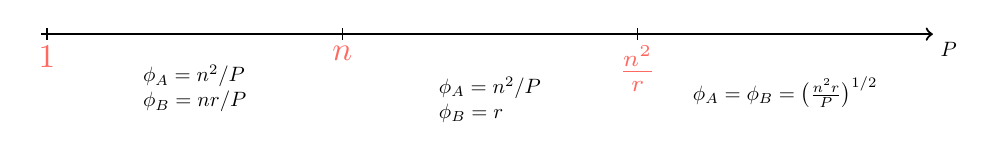
\begin{tikzpicture}[scale=0.75, every node/.style={transform shape}]
				%%\draw (-2,0) -- node[below] {a} ++(2,0) -- node[above] {b} ++(2,0);
				%%\draw (-0.1,0) -- ++(5,0) -- ++(5,0);
				\draw [->, thick] (-0.1,0) -- (15,0) node [below right] {$P$};
				\draw (0, 0.1) -- node [below, pastelred, scale=1.6]{$1$}(0,-0.1);
				\draw (5, 0.1) -- node [below, pastelred, scale=1.6]{$n$}(5,-0.1);
				\draw (10, 0.1) -- node [below, pastelred, scale=1.6] {$\frac{n^2}{r}$}(10,-0.1);
				
				\node[align=left,below] at (2.5, -0.4) {$\phi_A=n^2/P$\\ $\phi_B=nr/P$};
				\node[align=left,below] at (7.5, -0.6) {$\phi_A=n^2/P$\\$\phi_B=r$};
				\node[align=center,below] at (12.5, -0.6) {$\phi_A=\phi_B= \big(\frac{n^2r}{P}\big)^{1/2}$};	
				\end{tikzpicture}
			\end{center}
		\end{block}
	\vfill
	\end{frame}

	\begin{frame}{Our algorithm to compute $B=AV$ computation}
		\vspace*{-0.35cm}\begin{algorithm}[H]
			\caption{$B=AV$ computation}
			\begin{algorithmic}[1]
				\REQUIRE $A$, $p_1 \times p_2 \times p_3$ logical processor grid
				\ENSURE $B$ such that $B=AV$
				\STATE $(p_1^\prime, p_2^\prime, p_3^\prime)$ is my processor id
				\STATE $A_{p_1^\prime p_2^\prime}$ = All-Gather($A$, $(p_1^\prime, p_2^\prime, * )$)\label{alg:BAV:line:allGatherInputMatrix} \qquad\quad //All-gather input matrix $A$
%				\STATE //Generate random matrix of size $\frac{n}{p_2}\times \frac{r}{p_3}$
				\STATE $V_{p_2^\prime p_3^\prime}$ =  GenerateRequiredRandomMatrix() \quad\quad //Generate random matrix of size $\frac{n}{p_2}\times \frac{r}{p_3}$
				\STATE //Perform local computation in a temporary matrix $T$
				\STATE $T$ = $A_{p_1^\prime p_2^\prime} \cdot V_{p_2^\prime p_3^\prime}$
%				\STATE //Reduce-scatter the output matrix in $B_{p_1^\prime p_3^\prime}$
				\STATE Reduce-Scatter($B_{p_1^\prime p_3^\prime}$, $T$, $(p_1^\prime, *,  p_3^\prime)$) \qquad\quad //Reduce-scatter the output matrix in $B_{p_1^\prime p_3^\prime}$
			\end{algorithmic}
		\end{algorithm}
	\vfill
	Our algorithm is communication optimal when $p_1$, $p_2$ \& $p_3$ are chosen based on lower bounds.
	\vfill
	\end{frame}



	\begin{frame}{Compute lower bounds for $B=AV$ and $C=V^TAV$ }
		\vspace*{-0.25cm}$$B=AV \qquad \text{ and } \qquad C=V^TB$$
	\begin{itemize}
		\item Each processor performs $\frac{n^2r}{P}$ multiplications to compute $B$ and $\frac{nr^2}{P}$ multiplications to compute $C$
		\item Assume that same entries of $B$ are accessed on a processor for both computations
		\item After combining iteration spaces of both computations in a $6$-dimensional lattice, we need to solve the following optimization problem
	\end{itemize}
	\vspace*{-0.15cm}{\small\begin{align*}
		Minimize \ \phi_{A} + \phi_{B} + \phi_{C} \ & \text{ s.t.} \\
		\phi_{A} \phi_{B} \phi_{C} & \ge \frac{n^2r}{P}\cdot \frac{nr^2}{P} \\
		\frac{n^2}{P} \le  \phi_{A} \le n^2, \  
		\frac{nr}{P} \le & \phi_{B} \le nr, \ 
		\frac{r^2}{P} \le  \phi_{C} \le r^2, \ r\le n
		\end{align*}}

	\vspace*{-0.15cm}\begin{itemize}
		\item Can obtain communication lower bounds by solving the above optimization problem
		\item Similar to the previous algorithms, we can design communication optimal algorithms for a $p_1\times p_2 \times p_3$ logical processor grid 
	\end{itemize}
\vfill
\end{frame}

\subsection{Conclusion}
\begin{frame}{Outline}
	\tableofcontents[currentsubsection]
\end{frame}


\begin{frame}{Conclusion and future work}
	\begin{block}{Conclusion}
		\begin{itemize}
			\item Communication lower bounds and optimal algorithms for the computations of symmetric Nyström approximation
			%		\item Comparison of our approach with the TTM-in-Sequence approach
			\item An approach to obtain communication lower bounds for a set of computations
		\end{itemize}
	\end{block}
	\vfill
	\begin{block}{Future Work}
		\begin{itemize}
			\item Implementation of the proposed algorithms for real datasets
			\item Simplify and refine the lower bound computations
		\end{itemize}
	\end{block}
	\vfill
		\Huge{\centerline{Thank You!}}
\end{frame}

%\begin{frame}
%
%\end{frame}


\end{document} 